\chapter{MOLECULE SPECIFIC NORMALIZATION}

In this thesis, we propose a novel approach that adapts the normalization to each molecule. Our approach, called Molecule Specific Normalization (MSN), starts by identifying the candidate house-keeping molecules, i.e. molecules whose peak areas do not change significantly between sample groups, e.g. disease vs. control. The MSN algorithm aims to minimize the molecular profile difference of the house-keeping molecules across samples. Figure \ref{wf} depicts the work-flow of the proposed MSN method. After peak list alignment, molecules detected in all samples are organized in an alignment table, $P_{ki}$, with $k=1 \dots M$ molecules and $i=1 \dots N$ samples. The proposed method consists of two main steps: Initial Normalization and Iterative Sample Normalization Using Surface Fitting. 
\begin{figure}
	
	\centering
	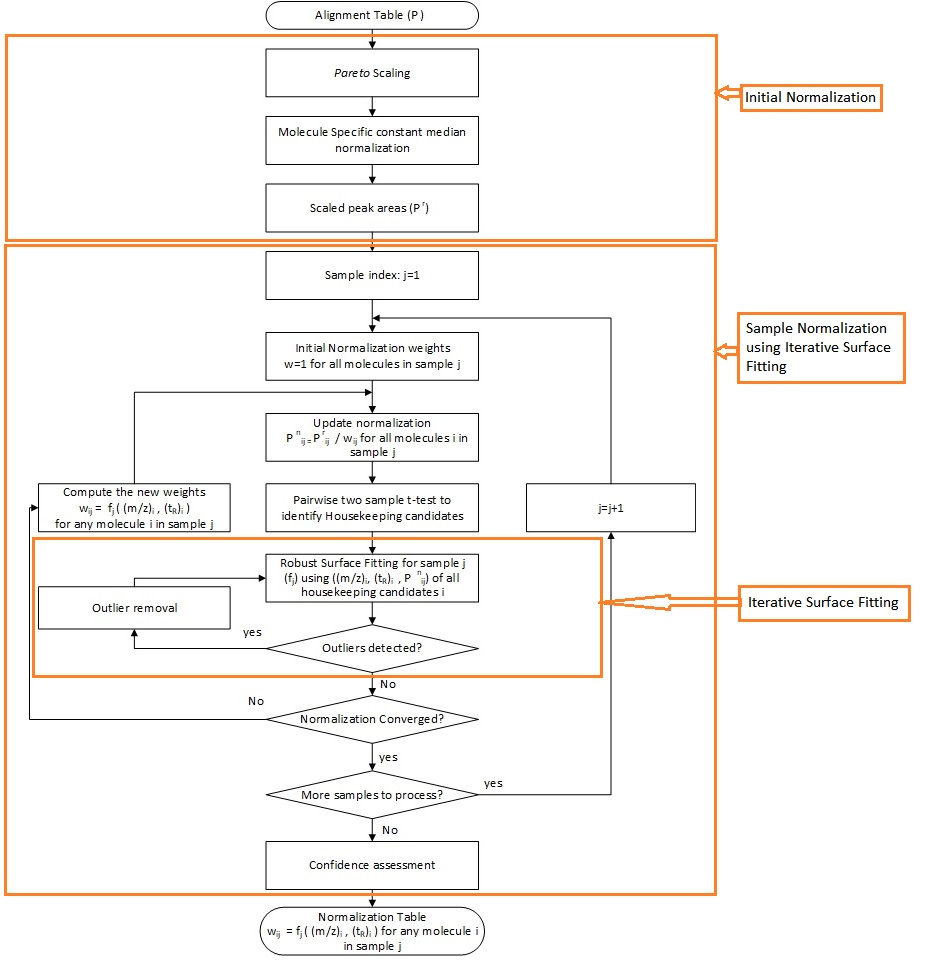
\includegraphics[width=1.1\textwidth]{Work_Flow3}
	\caption{Work flow of the proposed MSN method}
	\label{wf}
\end{figure}

\section{Initial Normalization}
The main aim of this step is to adjust for the differences in fold differences of peak areas between various molecules by converting the data into differences in peak area relative to the scaling factor. \\
\indent First, we apply Pareto Scaling \cite{berg:tar} to each sample across all molecules of the alignment table. Specifically, for each peak area in a selected sample, we apply the transformation:
\begin{eqnarray}\label{eq:0}
P_{ij}'= (P_{ij} - \mu ) / sqrt(s) 
\end{eqnarray}
where $\mu$ is the mean across all molecules of the selected sample and $s$ is the standard deviation of the peak areas of all molecules detected in that sample.\\
\indent After scaling, we proceed to normalize the abundance of each house-keeping molecule by the median of peak areas of that molecule across all samples. First, we compute the median ($Med_i$) of the peak area of a molecule (i) across all samples ($j=1,\dots ,N$). Then, the peak area ratio of each molecule is computed using:
\begin{eqnarray}\label{eq:2}
P_{ij}^r=P_{ij} / Med_i , \text{ $ i=1, \dots ,M$ and $j= 1, \dots ,N.$}
\end{eqnarray}
A table of ratios is then generated for all molecules $P^r$. This table will be used as input to the surface fitting in the next step.  Figure \ref{first_step} shows the selection of house-keeping molecules and median scaling steps.
\begin{figure}
	
	\centering
	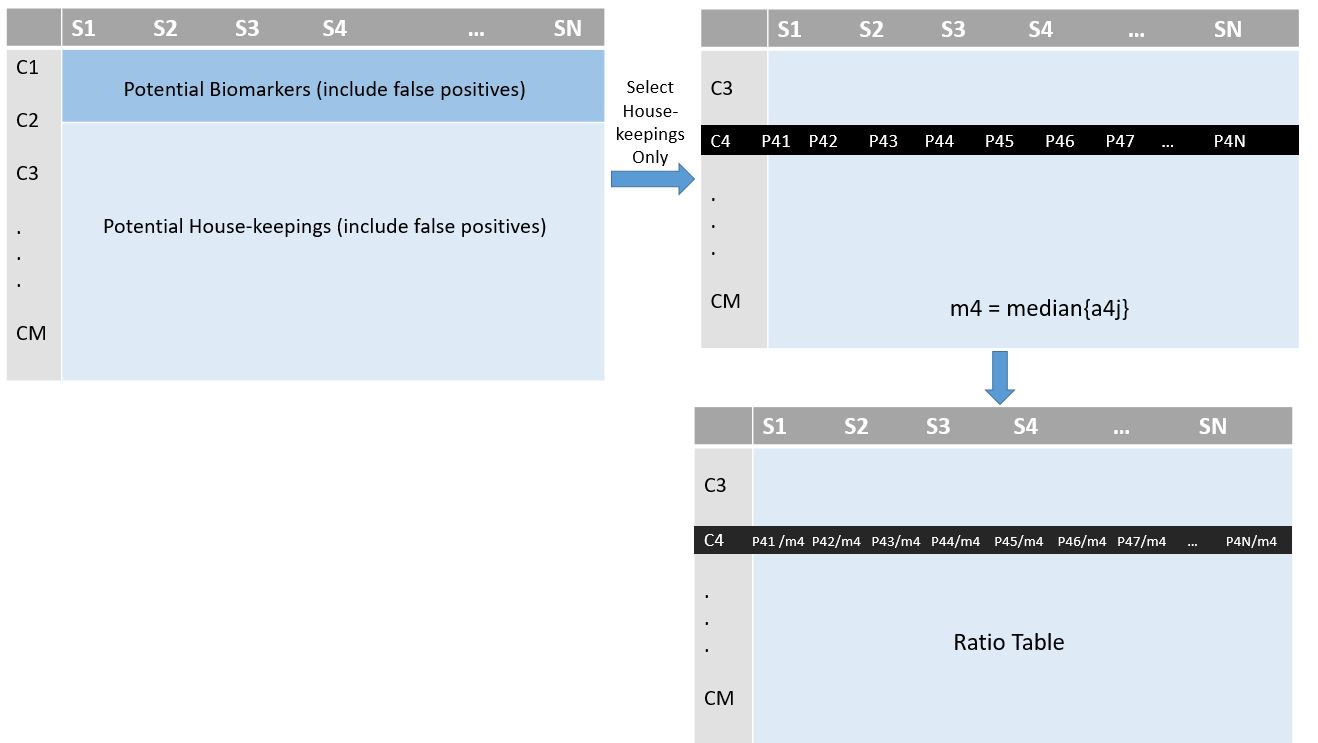
\includegraphics[width=1\textwidth]{first_step}
	\caption{Example of ratio table extraction}
	\label{first_step}
\end{figure}
\section{Sample Normalization Using Iterative Surface Fitting}
The next step of MSN is the main step of our proposed method and consists of sample normalization. The main goal of this step is to estimate weights for normalizing peak areas for all molecules.\\
\indent First, we randomly select one sample and  initialize the weights of all molecules in that sample to unity. These weights will be updated iteratively and the peak areas of the selected sample will be normalized by the updated weights at each iteration.\\
\indent Next, we identify potential house-keepings molecules by applying pairwise
two-tail t-test with sample permutation to deduce the p-value for each molecule. The t statistic for the t-test is computed using:
\begin{eqnarray} 
t={\frac {{\bar {P}}_{1}-{\bar {P}}_{2}}{s_{p}\cdot {\sqrt {{\frac {1}{n_{1}}}+{\frac {1}{n_{2}}}}}}}
\end{eqnarray}
where Sp is the pooled standard deviation
\begin{eqnarray}\label{het} 
 s_{p}={\sqrt {\frac {\left(n_{1}-1\right)s_{P_{1}}^{2}+\left(n_{2}-1\right)s_{P_{2}}^{2}}{n_{1}+n_{2}-2}}}.
\end{eqnarray}
\indent In \ref{het}, $s_{P_1}^2$ and $s_{P_2}^2$ are the unbiased estimators of the variances of the two samples. 
We select the house-keeping molecules as the set of molecules with p-value larger than $ \geq 0.05$. Note that the biomarkers are usually selected by setting $p <0.05$. In the following, we let $H$ denote the set of selected house-keeping molecules.\\
\indent After selecting the house-keepings, we proceed with the surface fitting step. This step will be detailed in section 3.3. \\
\indent After surface fitting, the normalization factor $w_{ij}$ of any molecule $i$ (including those that were not selected as the house-keeping candidates) in the j-th sample can be calculated from the j-th fitted surface function using its (m/z,$t_R$ ) values. The normalized peak area of this molecule is then calculated as:

\begin{eqnarray}\label{eq:3}
P_{ij}^f= P_{ij}^r / w_{ij}
\end{eqnarray}
Using the learned normalization factor $P_{ij}^f$ for the ith molecule in the jth sample, a pairwise t-test is reapplied to all molecules to identify an updated set of house-keeping molecules.
The fitting process for each sample will be repeated until the identified set of house-keepings do not change from iteration to iteration.

\begin{figure}
	
	\centering
	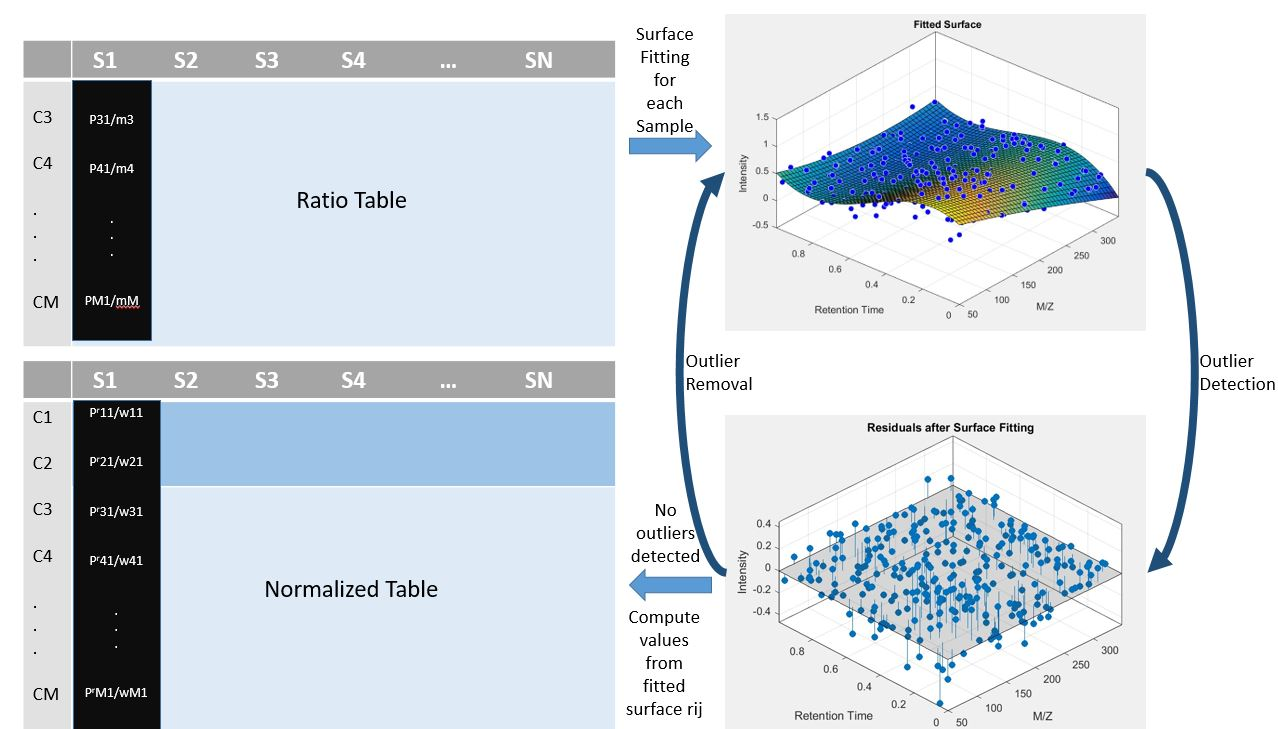
\includegraphics[width=1.1\textwidth]{second_step}
	\caption{Illustration of the iterative process of learning normalization weights and data normalization}
	\label{second_step}
\end{figure}

In Figure \ref{second_step}, we illustrate the iterative surface fitting and outlier detection and removal steps to learn the final normalization weights. 


\section{Robust Surface Fitting}

The main goal of this procedure is to estimate weights for normalizing peak areas for all molecules. To achieve this goal, we treat each sample separately and fit a surface to each one. For sample $j$, the two independent variables ($X$ , $Y$) to the surface fitting function include the m/z value and retention time, $t_R$, of each house-keeping molecule $h_i$. The dependent variable ($Z$) is the peak area ratio, $P^r_{ij}$. This component consists of two iterative steps. The first one fits the surface $ Z= f(X,Y)$. Initially, all house-keeping molecules are used for fitting. We use a Lowess local linear regression function for this step. The optimal fitting function is determined by using the Least Absolute Residual Robust method (LAR). The second iterative step consists of identifying molecules with large residual errors, i.e. outliers. These outliers are typically due to large variations introduced to the peak area of a molecule by random errors or technical variations. For instance, a chromatographic peak may be split into two peaks owing to its poor peak shape during spectrum deconvolution. This will result in a significantly reduced peak area for the low abundance molecules and therefore, a small peak area ratio and large variation in the residue after surface fitting. We use Box-plot for outlier detection since it does not assume residues to have a normal distribution.

The peak area ratios of the identified house-keeping outliers will be removed temporarily for the current fitting task and the remaining house-keeping molecules are used for the next iteration of surface fitting. This iterative process is repeated until no more house-keeping molecules can be detected as outliers. 

\chapter{OUTLIER DETECTION BASED ON FISHER CRITERION}
\indent The Fisher ratio \cite{fld} is used to measure the similarity of two objects on the basis of sets of measurements for each object and a statistical model. For the case of supervised learning, the class for a new object (whose real class is unknown) can be estimated by minimizing, across classes, an average of the Fisher kernel distance from the new object to each known member of the given class. In this thesis, we propose adapting the Fisher criterion to detect outliers.\\
\indent First, we assume the training data belongs to two classes, and in each class $i$ we have $n_i$ samples $P_{n,i}, n=1,\dots , n_i$. The mean of each class is computed using:
\begin{eqnarray}
{\mathbf  {m}}_{i}={\frac  {1}{n_{i}}}\sum _{{n=1}}^{{n_{i}}}{\mathbf  {P}}_{n,i},
\end{eqnarray}
The Fisher Ratio is defined as:
\begin{eqnarray}\label{ratio}
J={\frac  {{\mathbf  {S}}_{B}}{{\mathbf  {S}}_{W}}},
\end{eqnarray}
where $S_B$ is the between class scatter matrix:
\begin{eqnarray}
{\mathbf  {S}}_{B}&=({\mathbf  {m}}_{2}-{\mathbf  {m}}_{1})({\mathbf  {m}}_{2}-{\mathbf  {m}}_{1})^{{{\text{T}}}}
\end{eqnarray}
and $S_W$ is the within class scatter matrix:
\begin{eqnarray}
{\mathbf  {S}}_{W}&=\sum _{{i=1,2}}\sum _{{n=1}}^{{l_{i}}}({\mathbf  {P}}_{n,i}-{\mathbf  {m}}_{i})({\mathbf  {P}}_{n,i}-{\mathbf  {m}}_{i})^{{{\text{T}}}}
\end{eqnarray}


The proposed approach focuses on the similarity among the samples (the replicas) of each class. If there are no outliers, the scatter matrix and thus the ratio will be ideally constant even if we delete one sample from either classes since the information contained in one sample is replicated in all the replicas. On the contrary, if one sample is an outlier, the ratio before deleting this sample will be very different from the ratio after deleting the sample. \\
\indent To illustrate this idea, suppose we have one feature $F1$ in two classes $C1$ and $C2$ where $F_1^{C1}=[f_{c1}^1,f_{c1}^2 \ldots f_{c1}^{n1} ]$ are the samples of feature $F1$ in $C1$, and $F_1^{C2}=[f_{c2}^1,f_{c2}^2 \ldots f_{c2}^{n2} ]$ are the samples of feature $F1$ in $C2$. First, we use equation (\ref{ratio}) to compute the fisher ratio each time  one sample from $C2$ is deleted . This will result in $n_2$ ratios $R=[J_1, J_2 ... J_{n2}]$ where $J_k$ is the fisher ratio after deleting the $k^{th}$ sample $f_{c2}^k$. \\

Ideally, if there are no outliers in class $C2$, all ratios within $R$ should be equal. However, in practice, the samples are not identical, and the ratios should form a distribution. The idea is to identify samples that result in Fisher ratios that do not fit the distribution and label them as outliers. In fact, if one sample (or more) is an outlier then after deleting it, the ratio will change remarkably from the distribution formed by the other ratios. Since we cannot assume that ratios within $R$ fit a known distribution, we use the Boxplot method (chapter 2) to detect the outliers.\\
Figure ~\ref{fish} illustrates our approach to detect outliers based on Fisher Criterion. The Figure includes three examples of detected outliers in compounds with noise added to their samples in class $C2$. The first example is a compound with no outliers detected after applying our algorithm. The second example is when one outlier was detected using our algorithm and the third is when two outliers were detected.\\
\indent The plots on the left of the Figure are the data points of one compound in the two classes $C1$ and $C2$ with noise added to class $C2$.
The plots on the right are the distributions formed by the ratios for different features. The ratios are calculated each time after retrieving one data sample. The red points circled in orange are the points that were selected as outliers from the distribution using Boxplot. The y axis is the ratio value.\\
\indent  One main advantage of our proposed method is that it is applicable to any data with unknown distribution. The absence of  normal distribution or any specific distribution assumption gives it a favor compared to other methods such as Grubbs, GESD and Kimber in terms of applicability. Compared to boxplot, which is a method that is also independent from any distribution assumption, we will show that our method is better in terms of efficiency and classification improvement.
\begin{figure}[t!]
	\centering
	\begin{subfigure}{1\textwidth}
		\centering
		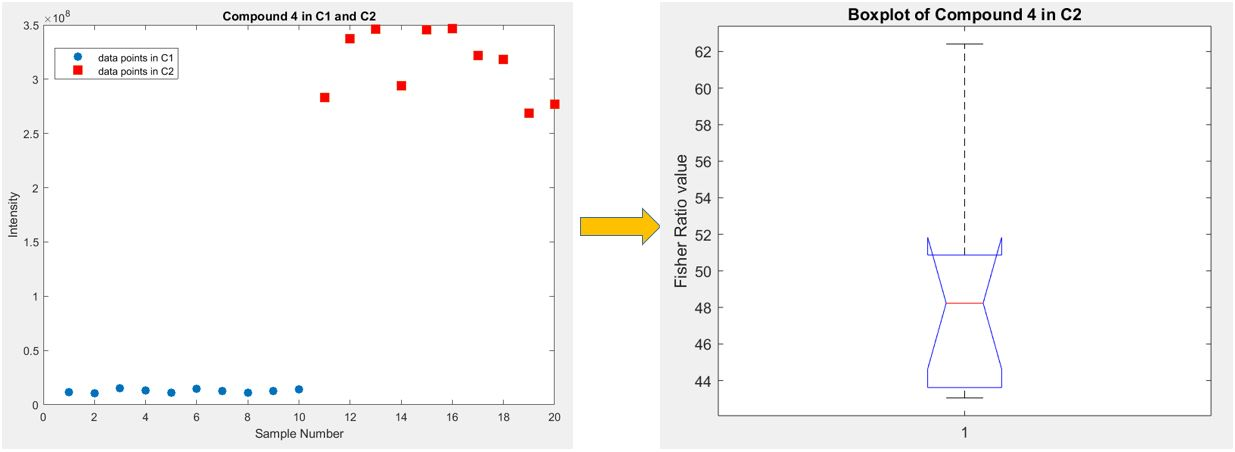
\includegraphics[height=2.1in]{no_outlier}
		\caption{Example 1 with no outlier detected in $C2$}
		\label{fisher1}
	\end{subfigure}%
	 \\
	\begin{subfigure}{1\textwidth}
		\centering
		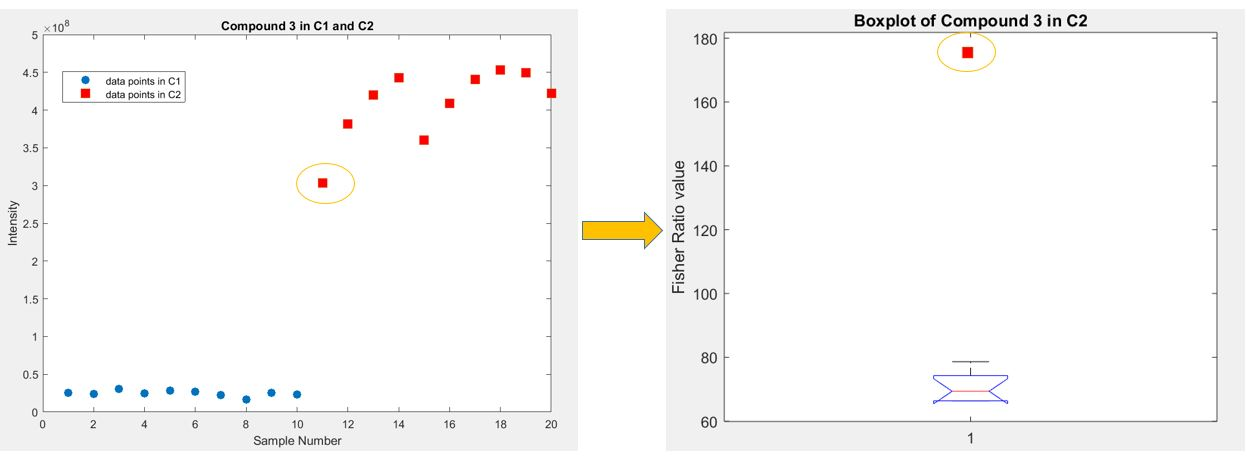
\includegraphics[height=2.1in]{one_outlier}
		\caption{Example 2 with one outlier detected in $C2$}
		\label{fisher2}
	\end{subfigure}

	\begin{subfigure}{1\textwidth}
		\centering
		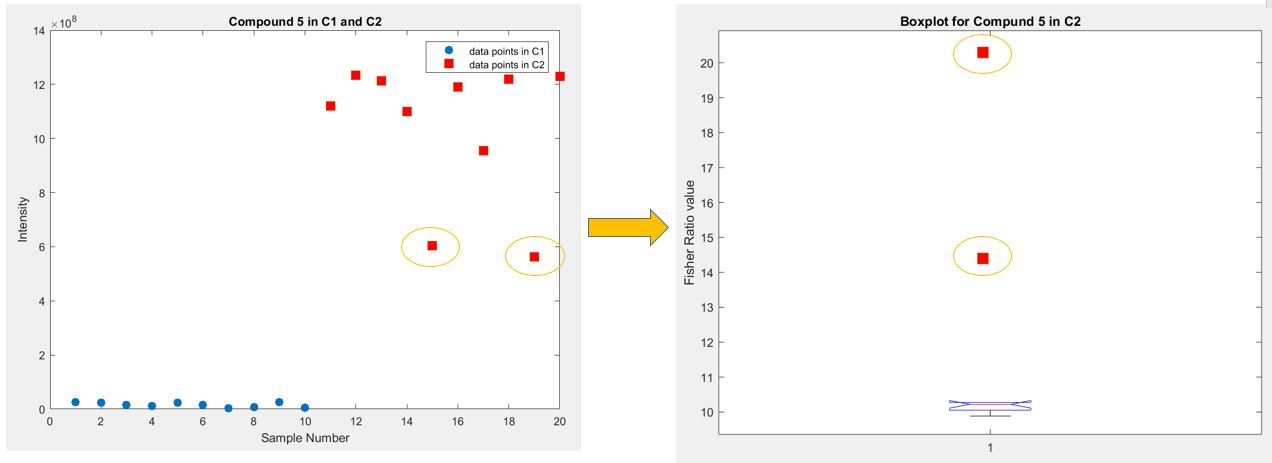
\includegraphics[height=2.1in]{two_outlier}
		\caption{Example 3 with two outlier detected in $C2$}
		\label{fisher3}
	\end{subfigure}
	\caption{Examples of detected outliers in compounds with noise added to their samples in class $C2$}
	\label{fish}
\end{figure}
